\documentclass[12pt,b5paper]{ltjsarticle}

%\usepackage[margin=15truemm, top=5truemm, bottom=5truemm]{geometry}
%\usepackage[margin=10truemm,left=15truemm]{geometry}
\usepackage[margin=10truemm]{geometry}

\usepackage{amsmath,amssymb}
%\pagestyle{headings}
\pagestyle{empty}

%\usepackage{listings,url}
%\renewcommand{\theenumi}{(\arabic{enumi})}

%\usepackage{graphicx}

\usepackage{tikz}
%\usetikzlibrary {arrows.meta}
%\usepackage{wrapfig}
\usepackage{bm}

% ルビを振る
%\usepackage{luatexja-ruby}	% required for `\ruby'

%% 核Ker 像Im Hom を定義
%\newcommand{\Img}{\mathop{\mathrm{Im}}\nolimits}
%\newcommand{\Ker}{\mathop{\mathrm{Ker}}\nolimits}
%\newcommand{\Hom}{\mathop{\mathrm{Hom}}\nolimits}

%\DeclareMathOperator{\Rot}{rot}
%\DeclareMathOperator{\Div}{div}
%\DeclareMathOperator{\Grad}{grad}
%\DeclareMathOperator{\arcsinh}{arcsinh}
%\DeclareMathOperator{\arccosh}{arccosh}
%\DeclareMathOperator{\arctanh}{arctanh}

\usepackage{url}

%\usepackage{listings}
%
%\lstset{
%%プログラム言語(複数の言語に対応,C,C++も可)
%  language = Python,
%%  language = Lisp,
%%  language = C,
%  %背景色と透過度
%  %backgroundcolor={\color[gray]{.90}},
%  %枠外に行った時の自動改行
%  breaklines = true,
%  %自動改行後のインデント量(デフォルトでは20[pt])
%  breakindent = 10pt,
%  %標準の書体
%%  basicstyle = \ttfamily\scriptsize,
%  basicstyle = \ttfamily,
%  %コメントの書体
%%  commentstyle = {\itshape \color[cmyk]{1,0.4,1,0}},
%  %関数名等の色の設定
%  classoffset = 0,
%  %キーワード(int, ifなど)の書体
%%  keywordstyle = {\bfseries \color[cmyk]{0,1,0,0}},
%  %表示する文字の書体
%  %stringstyle = {\ttfamily \color[rgb]{0,0,1}},
%  %枠 "t"は上に線を記載, "T"は上に二重線を記載
%  %他オプション:leftline,topline,bottomline,lines,single,shadowbox
%  frame = TBrl,
%  %frameまでの間隔(行番号とプログラムの間)
%  framesep = 5pt,
%  %行番号の位置
%  numbers = left,
%  %行番号の間隔
%  stepnumber = 1,
%  %行番号の書体
%%  numberstyle = \tiny,
%  %タブの大きさ
%  tabsize = 4,
%  %キャプションの場所("tb"ならば上下両方に記載)
%  captionpos = t
%}

%\usepackage{cancel}
%\usepackage{bussproofs}
%\usepackage{proof}



\begin{document}

\hrulefill


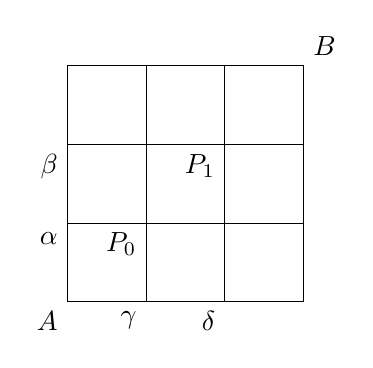
\begin{tikzpicture}[scale=1]

\draw (0,0) -- (3,0) -- (3,1) -- (0,1) -- (0,2) -- (3,2) -- (3,3) -- (0,3);
\draw (0,0) -- (0,3) -- (1,3) -- (1,0) -- (2,0) -- (2,3) -- (3,3) -- (3,0);

\node [below left] (A) at (0,0) {$A$};

\node [below left] (Y1) at (0,1) {$\alpha$};
\node [below left] (Y2) at (0,2) {$\beta$};
\node [below left] (X1) at (1,0) {$\gamma$};
\node [below left] (X2) at (2,0) {$\delta$};

\node [below left] (X1Y1) at (1,1) {$P_{0}$};
\node [below left] (X2Y2) at (2,2) {$P_{1}$};

\node [above right] (B) at (3,3) {$B$};

\end{tikzpicture}


点$A$から点$B$まで最短距離で移動する場合


点$\alpha$に来るには
$A$からのみであるから、
$\alpha$へ到達する確率は
$A$から2通りの分岐(上と右)のうち上のみであるので、
$1/2$となる。

点$\beta$に来るには$\alpha$からのみであり、
$\alpha$からは分岐(上と右)があるので、
$\beta$へ到達する確率は
$\alpha$に到達する確率に$1/2$をかけたものになる。

同様に$\gamma,\delta$も考えると
それぞれの地点に到達する確率は
$\alpha=1/2,\;\beta=1/4,\;\gamma=1/2,\;\delta=1/4$
となる.

$P_{0}$に到達するには、
$\alpha$から来る道と$\gamma$から来る道がある。
それぞれが、上と右の分岐があるので、
$P_{0}$に来る確率は次のようになる。
\begin{equation}
 \overset{\alpha \text{の確率}}{\frac{1}{2}}\times \overset{\text{2択の1つ}}{\frac{1}{2}}
 +
 \overset{\gamma \text{の確率}}{\frac{1}{2}}\times \overset{\text{2択の1つ}}{\frac{1}{2}}
 = \frac{2}{4}
\end{equation}


同様に$P_{1}$に来る確率は
$P_{1}$の左の点に来る確率に$1/2$をかけたものと
$P_{1}$の下の点に来る確率に$1/2$をかけたものを足したものとなる。

\begin{equation}
 \overset{\text{左}}{\frac{3}{8}}\times \overset{\text{2択}}{\frac{1}{2}}
 +
 \overset{\text{下}}{\frac{3}{8}}\times \overset{\text{2択}}{\frac{1}{2}}
 = \frac{3}{8}
\end{equation}




\hrulefill

\end{document}
